\begin{figure}[H]
    \centering
    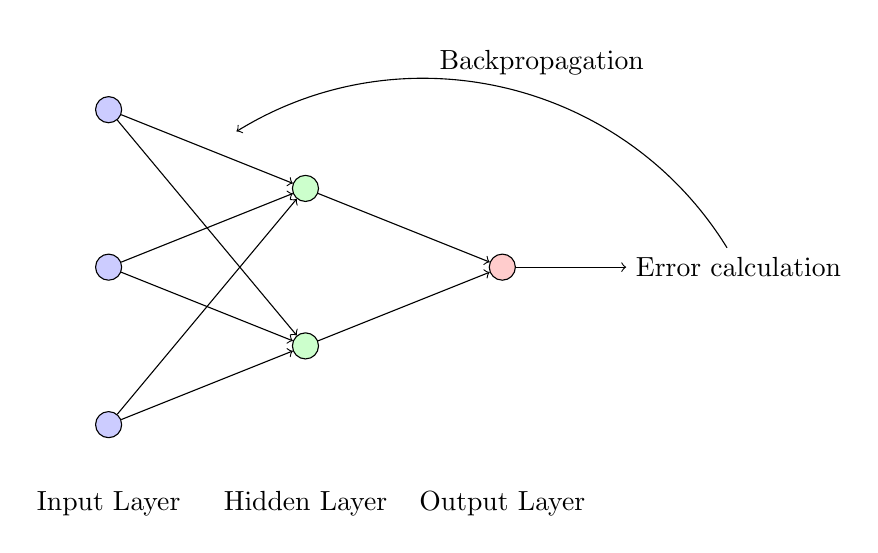
\begin{tikzpicture}
        \node[circle, draw, fill=blue!20] (I1) at (0,4) {};
        \node[circle, draw, fill=blue!20] (I2) at (0,2) {};
        \node[circle, draw, fill=blue!20] (I3) at (0,0) {};
        \node (I4) at (0,-1) {Input Layer};
        \node[circle, draw, fill=green!20] (H1) at (2.5,3) {};
        \node[circle, draw, fill=green!20] (H2) at (2.5,1) {};
        \node (H3) at (2.5,-1) {Hidden Layer};
        \node[circle, draw, fill=red!20] (O1) at (5,2) {};
        \node (O2) at (5,-1) {Output Layer};
        \foreach \i in {1,2,3}
            \foreach \j in {1,2}
                \draw[->] (I\i) -- (H\j);
        \foreach \i in {1,2}
            \draw[->] (H\i) -- (O1);
        \node (B1) at (8, 2) {Error calculation};
        \draw[->] (O1) -- (B1);
        \node (B2) at (1.5, 3.65) {};
        \draw[->] (B1) to [bend right=45] (B2);
        \node (B3) at (5.5, 4.6) {Backpropagation};
    \end{tikzpicture}
    \caption{Backpropagation in action within a simple neural network.}
    \label{fig:backpropagation}
\end{figure}